\documentclass[12pt, a4paper]{article}

\usepackage[spanish]{babel}
\usepackage{amsmath}
\usepackage[labelfont=bf]{caption}

\usepackage{hyperref}
\hypersetup{
    colorlinks,
    citecolor={red!50!black},
    linkcolor={blue!50!black},
    urlcolor={blue!80!black}
}

\usepackage{mathtools}
\usepackage{multicol}
% \usepackage{esvect}
\usepackage{physics}
\usepackage{parskip}

% Circuitikz
\usepackage[american, RPvoltages]{circuitikz}
\usetikzlibrary{calc}
\usetikzlibrary{patterns}
\ctikzset{quadpoles/fourport/height=3}
\ctikzset{quadpoles/fourport/width=1.5}
% \ctikzset{bipoles/length=0.8cm}
% \ctikzset{bipoles/diode/height=.375}
% \ctikzset{bipoles/diode/width=.3}
% \ctikzset{tripoles/thyristor/height=.8}
% \ctikzset{tripoles/thyristor/width=1}
% \ctikzset{bipoles/vsourceam/height/.initial=.7}
% \ctikzset{bipoles/vsourceam/width/.initial=.7}
% \tikzstyle{every node}=[font=\small]
% \tikzstyle{every path}=[line width=0.8pt,line cap=round,line join=round]


% Bold vectors
\renewcommand{\vec}[1]{\mathbf{#1}}
\makeatletter
\newcommand{\vv}[2][]{
    \@ifempty{#1}{\vec{#2}}{\vec{#2}_{#1}}
}
\makeatother

\title{Apuntes de Sistemas Electroacústicos}
\author{Javier Rodrigo López}
\date{\today}
 

%%%%%%%%%%%%%%%%%%%%%%%%%%%%%%%%%%%%%%%%%%%%%%%%%%%%%
\begin{document}
% \renewcommand{\arraystretch}{1.2}
\maketitle

% Table of contents
\tableofcontents

\newpage
\section*{Introducción}

\section{Altavoces}

\subsection{Introducción al altavoz electrodinámico}


Un altavoz se compone de varios elementos:

\begin{itemize}
    \item Imán
    \item Bobina
    \item Membrana, cono o diafragma
    \item Bornas de conexión (entre la membrana y la bobina)
\end{itemize}

A bajas frecuencias se puede aproximar al comportamiento de un pistón, pero a altas frecuencias pueden aparecer resonancias. 

\subsubsection{Sección eléctrica}

\begin{figure}
    \centering
    \begin{circuitikz}[scale=0.8, transform shape]
        \draw (0,0) node[fourport, anchor=port1] (A) {};
        \coordinate (A1) at (A.port1);
        \coordinate (A4) at (A.port4);

        \draw (3,0) node[fourport, anchor=port1] (B) {};

        \draw (6,0) node[fourport, anchor=port1] (C) {};
        \draw (9,0) node[fourport, anchor=port1] (D) {};
        \draw (12,0) node[fourport, anchor=port1] (E) {};

        
        \draw (A1) to ++(-2,0) node(corner){} to[sV, v=$ $, l_=$e_g$] (corner|-A4) to[R, l=$R_e$] (A4);
        
        % Líneas de abajo
        \draw (A.port2) to (B.port1);
        \draw (B.port2) to (C.port1);
        \draw (C.port2) to (D.port1);
        \draw (D.port2) to (E.port1);
        % Líneas de arriba
        \draw (A.port3) to (B.port4);
        \draw (B.port3) to (C.port4);
        \draw (C.port3) to (D.port4);
        \draw (D.port3) to (E.port4);

        % Draw labels on center of fourports
        \node[align=center] at (A.center) {Sección\\eléctrica};
        \node[align=center] at (B.center) {Sección\\electro-\\mecánica};
        \node[align=center] at (C.center) {Sección\\mecánica};
        \node[align=center] at (D.center) {Sección\\mecánico-\\acústica};
        \node[align=center] at (E.center) {Sección\\acústica};

        % Draw underbrace
        \node[align=center] at (-1.1,-0.5) (hola) {$\underbrace{\phantom{holaaaaaa}}_{\text{Amplificador}}$};

    \end{circuitikz}
    \caption{Modelo de altavoz electrodinámico}
\end{figure}

\subsubsection{Sección de conversión electromećanica}

\subsubsection{Sección mecánica}

Las partes mécanicas del altavoz son la membrana y la araña (suspensión). En términos de mecánica, este sistema es equivalente a un pistón, un muelle y una masa. VER DIAGRAMA CUADERNO

\begin{equation} \label{eq:ley_hooke}
    F = -kz
\end{equation}

\begin{equation} \label{eq:amortiguamiento}
    F = -d \dv{z}{t}
\end{equation}

Donde $d$ es la disipación de energía por rozamiento.

\begin{equation} \label{eq:masa}
    F = m \dv[2]{z}{t}
\end{equation}

\begin{equation} \label{eq:ecuacion_seccion_mecanica}
    F - k z - d \dv{z}{t} = m \dv[2]{z}{t}
\end{equation}

\begin{equation} \label{eq:ecuacion_seccion_mecanica_2}
    F = kz + d \dv{z}{t} + m \dv[2]{z}{t}
\end{equation}

\subsubsection{Sección de conversión mecánico-acústica}

Para hallar la impedancia de radiación, recordamos que una impedancia es la relación entre tensión y corriente. En nuestro modelo, la tensión se relaciona con la velocidad y la corriente con la fuerza. Por lo tanto, la impedancia de radiación es la relación entre la velocidad de la membrana y la fuerza que se ejerce sobre ella.

La impedancia acústica mide cuánto se está oponiendo el medio acústico (aire) al movimiento del pistón. El pistón comprime y expande el aire y genera una variación de la presión.

\begin{equation} \label{eq:incremento_presion}
    \dd p_1 = j\omega\rho_0 v_z d S_1 \frac{e^{-jkr_1}}{2\pi r_1}
\end{equation}

Una región 1 del pistón genera una fuerza sobre otra región 2 del pistón de la siguiente manera: 
\begin{equation} \label{eq:presion_de_1_sobre_2}
    \dd f_{1,2} = j\omega \rho_0 v_z d S_1 \frac{e^{-jkr_1}}{2\pi r_1} \dd S_2
\end{equation}

\begin{equation} \label{eq:presion_de_2_sobre_1}
    F = \frac{j\omega \rho_0 v_z}{2\pi} \int_{S_1} \int_{S_2} \frac{e^{-jkr_{1,2}}}{r_{1,2}} \dd S_1 \dd S_2    
\end{equation}

La solución de esta ecuación es:

\begin{equation} \label{eq:impedancia_piston}
    Z_{ac} = \frac{F}{v_z} = \pi a^2 \rho_0 c \left[ \left( 1 - \frac{J_1 (2ka)}{ka}  \right) + j \left( \frac{H_1 (2ka)}{ka} \right)\right]
\end{equation}

Donde $J_1$ y $H_1$ son la función de Bessel de primer tipo y orden 1 y la función de Struve de primer tipo y orden 1, respectivamente. Podemos ver la representación de la impedancia de radiación en la \autoref{fig:impedancia_radiacion}.

\begin{figure}[htp]
    \centering
    \caption{Impedancia de radiación acústica de un pistón}
    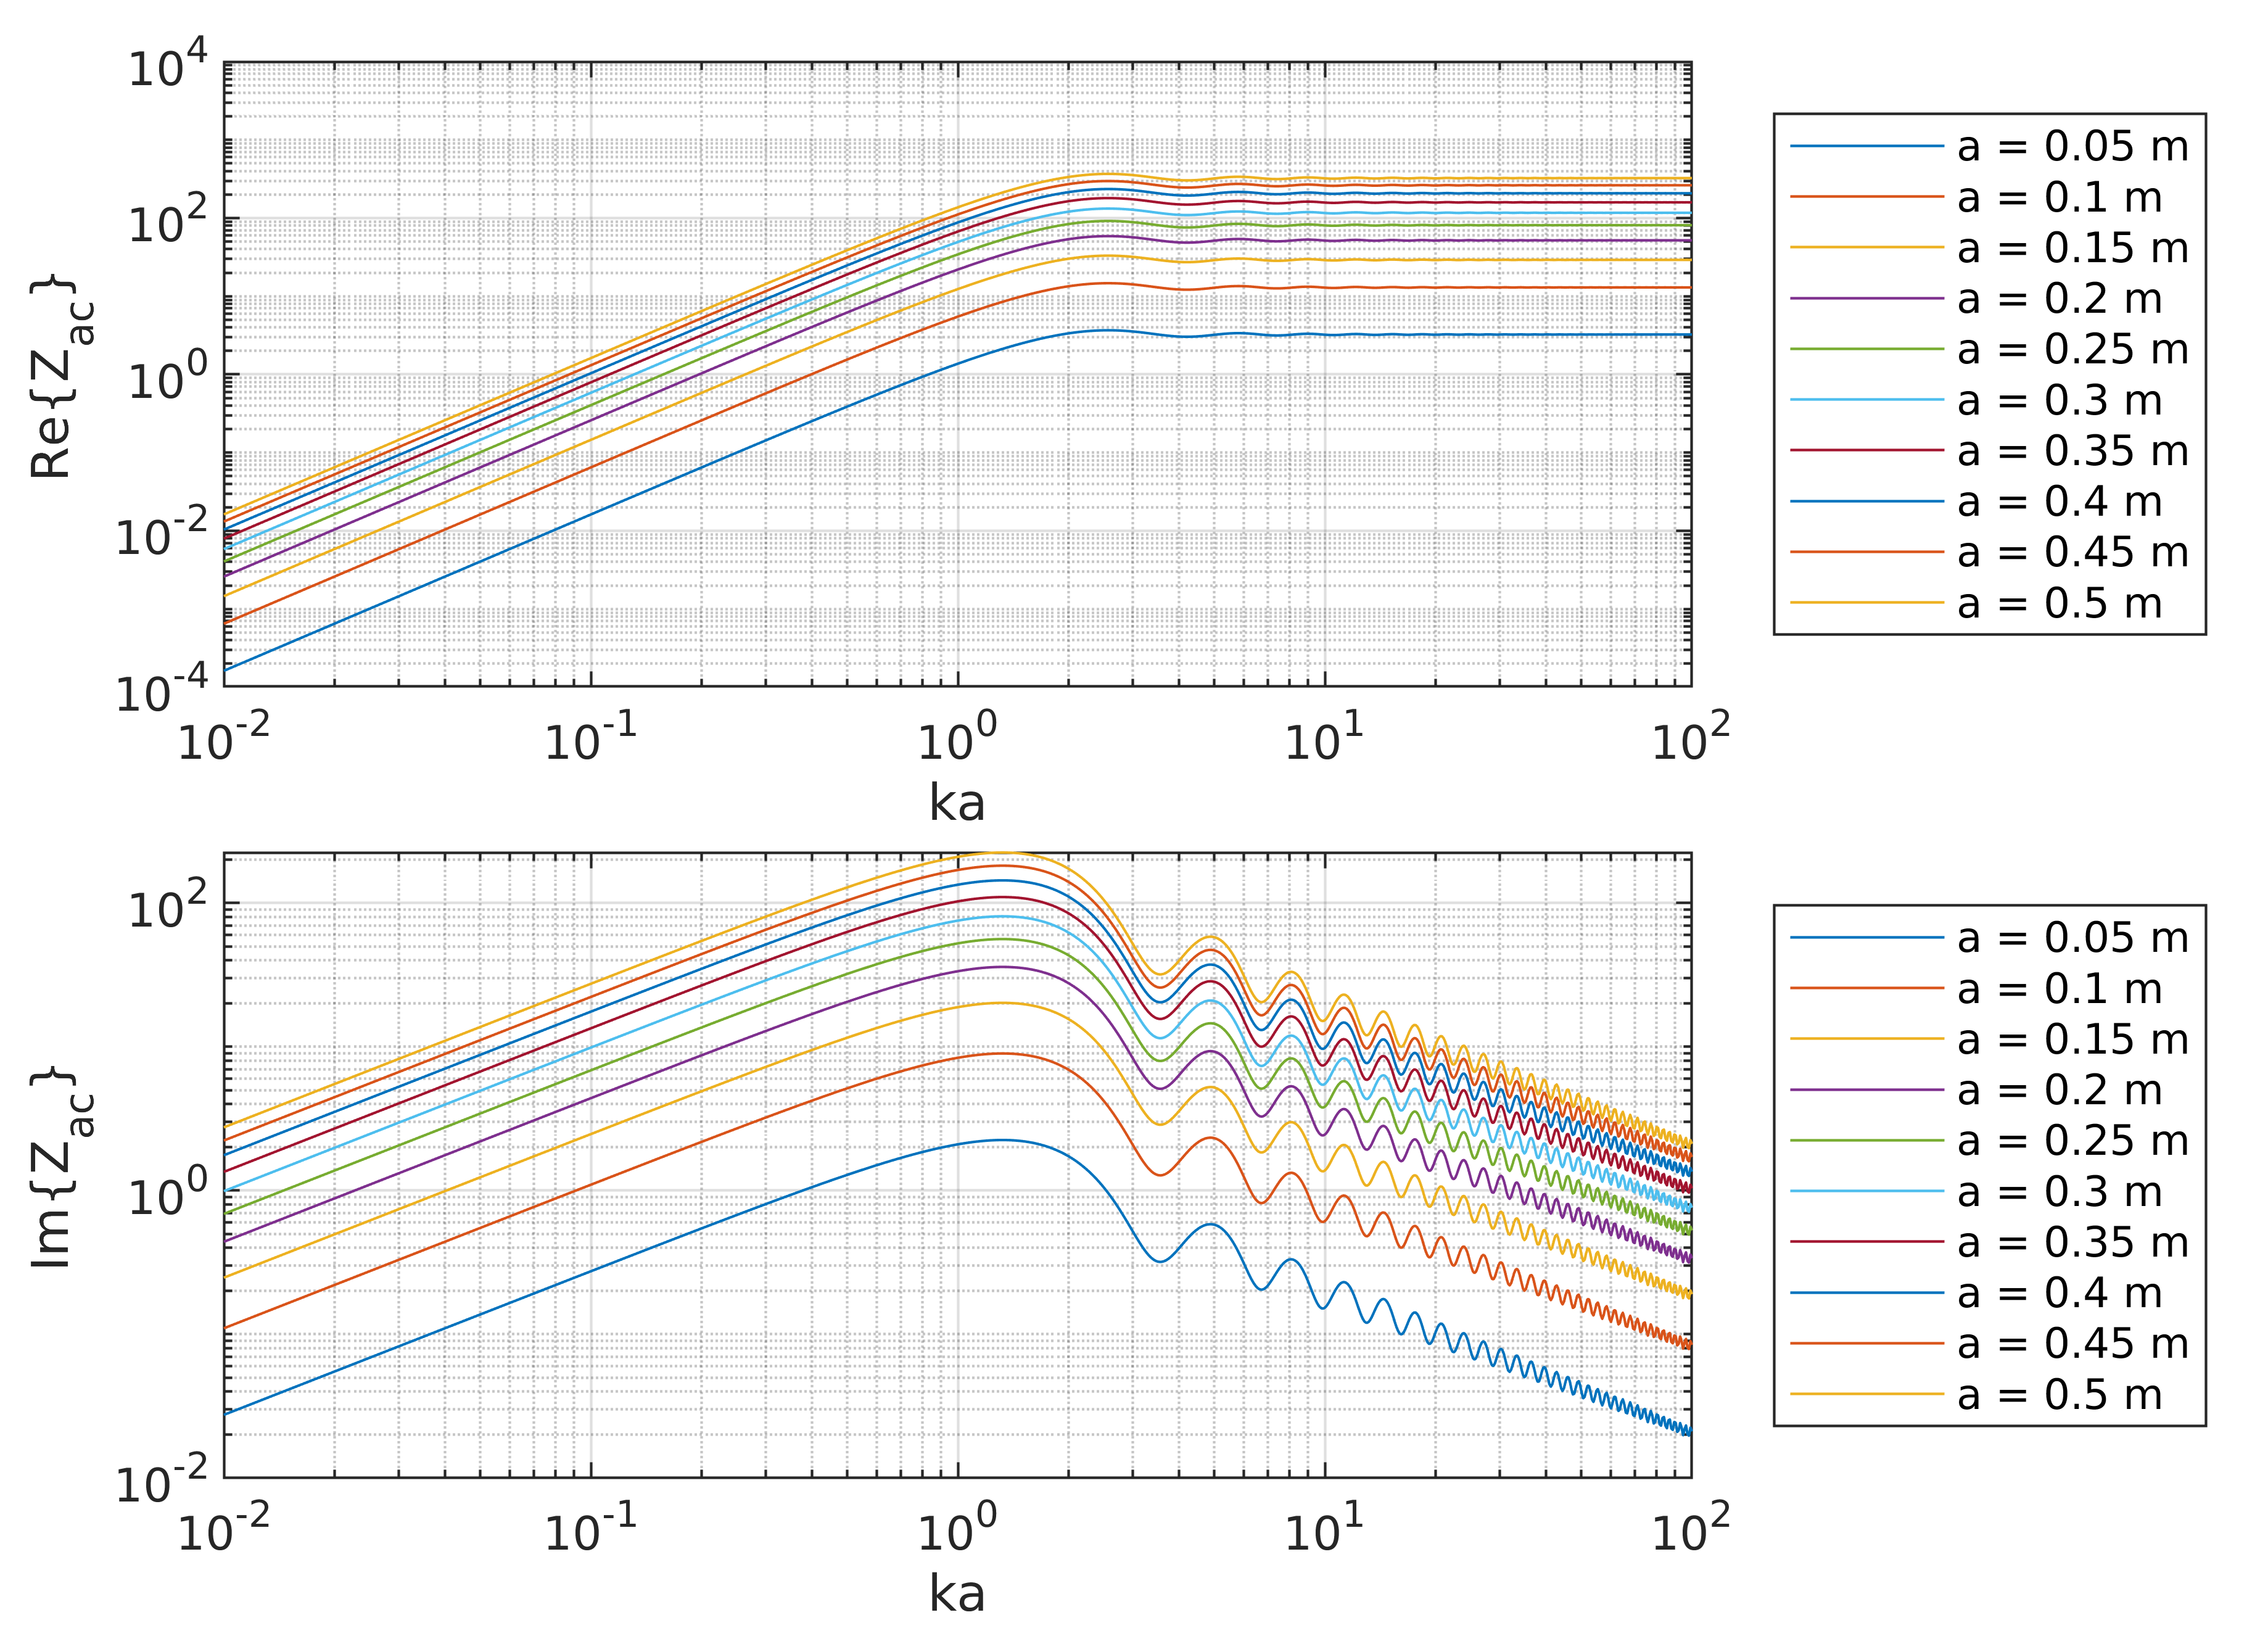
\includegraphics[width=\linewidth]{images/acoustic_radiation_impedance.png}
\label{fig:impedancia_radiacion}
\end{figure}



\subsubsection{Modelo completo del altavoz}

INSERTAR DIAGRAMA CIRCUITO

\begin{figure}[htp]
    \centering
    \caption{Modelo eléctrico completo del altavoz}
    \begin{circuitikz}
        \draw (0,0) to[sV, v=$e_g'$] ++(0,3) to[R=$R_E'$] ++(3,0) to[L=$L_E'$] ++(2,0) 
        ;
    \end{circuitikz}
\label{fig:modelo_completo_altavoz}
\end{figure}

\begin{align*}
    e'_g &= \frac{e_g}{Bl} & R_{MS} &= \frac{1}{d} & R_{AP-LF} &= \frac{1}{2} \cdot \frac{9\pi}{\rho_0ca^2} \\
    R'_E &= \frac{R_g+R_E}{\left( Bl \right)^2} & C_{MS} &= \frac{1}{k} & R_{AP-HF} &= \frac{1}{2} \cdot \frac{1}{\rho_0c\pi a^2} \\
    L'_E &= \frac{L_E}{\left( Bl \right)^2} & M_{MS} &= m & M_{AP} &= 2 \cdot \frac{8}{3} \rho_0 a^3 \\
\end{align*}

A \textbf{baja frecuencia}, la impedancia de radiación es fundamentalmente capacitiva.

Tras calcular la $Z_{\text{eq}}$ (ver cuaderno), podemos ver que el sistema se comporta como un filtro paso banda. La función de transferencia del sistema queda así:
\begin{equation} \label{eq:funcion_transferencia_altavoz_LF}
    H_{LF}(s) = \frac{H_0 s }{s^2 + \frac{\omega s }{Q } + \omega_s^2}
\end{equation}

\begin{equation} \label{eq:impedancia_altavoz_LF}
    Z_{LF}(s) = \frac{\frac{1}{C_{\text{eq}}s}}{s^2 + \frac{1}{C _{\textnormal{eq}R_{MS}}}s + \frac{1}{C_{\text{eq}}C_{MS}}}
\end{equation}

\begin{equation} \label{eq:f_res_LF}
    \omega_s = \frac{1}{\sqrt{C_{\text{eq}}C_{MS}}}
\end{equation}

Como $\frac{1}{Q _{\text{eq}}} = \frac{\omega_s}{Q}$, entonces:
\begin{equation} \label{eq:factor_calidad}
    Q = \omega_s R_{MS} C _{\text{eq}} = R_{MS} \sqrt{\frac{C _{\text{eq}}}{C_{MS}}}
\end{equation}

Donde $Q$ es el factor de calidad del sistema correspondiente a la parte mecánica y acústica.

La impedancia máxima que ve el sistema es $R_d$ a la frecuencia de resonancia.

La impedancia eléctrica total será:
\begin{equation} \label{eq:impedancia_electrica}
    Z_E = R_E + \frac{\left( Bl \right)^2 \frac{1}{C _{\text{eq}}}s}{s^2 + \frac{1}{R_{MS}C _{\text{eq}}}s + \frac{1}{C _{\text{eq}}C_{MS}}}
\end{equation}

Este sistema, que tiene en cuenta también la parte eléctrica del altavoz, tendrá un factor de calidad diferente que llamaremos \textbf{factor de calidad total} $Q_t$ y que será:
\begin{equation} \label{eq:factor_calidad_total}
    Q_t = ?
\end{equation}


\begin{figure}[htp]
    \centering
    \caption{Modelo del altavoz a alta frecuencia}
    \begin{circuitikz}
        \draw (0,0) to[sV, v=$e_g'$]  ++(0, 3) to[L=$L_E'$, -*] ++(3,0) node(n1){} to[short, -*] ++(2,0) node(n2){} to[R=$R_{AP-HF}$] ++(3,0) to[short] ++(0,-3) to[short, -*] ++(-3,0) node(n3){} to[C, l_=$M_{MS}$, -|] (n2.center);
        \draw (n3.center) to[short, -*] ++(-2,0) node(n4){} to[R=$R_{MS}$] (n1.center);
        \draw (n4.center) to[short] (0,0);
        \draw (n4) to[open] ++(1,0) node[ground]{};
    \end{circuitikz}
\label{fig:altavoz_HF}
\end{figure}

A \textbf{alta frecuencia}




\end{document}